% Options for packages loaded elsewhere
\PassOptionsToPackage{unicode}{hyperref}
\PassOptionsToPackage{hyphens}{url}
\PassOptionsToPackage{dvipsnames,svgnames,x11names}{xcolor}
%
\documentclass[
]{agujournal2019}

\usepackage{amsmath,amssymb}
\usepackage{iftex}
\ifPDFTeX
  \usepackage[T1]{fontenc}
  \usepackage[utf8]{inputenc}
  \usepackage{textcomp} % provide euro and other symbols
\else % if luatex or xetex
  \usepackage{unicode-math}
  \defaultfontfeatures{Scale=MatchLowercase}
  \defaultfontfeatures[\rmfamily]{Ligatures=TeX,Scale=1}
\fi
\usepackage{lmodern}
\ifPDFTeX\else  
    % xetex/luatex font selection
\fi
% Use upquote if available, for straight quotes in verbatim environments
\IfFileExists{upquote.sty}{\usepackage{upquote}}{}
\IfFileExists{microtype.sty}{% use microtype if available
  \usepackage[]{microtype}
  \UseMicrotypeSet[protrusion]{basicmath} % disable protrusion for tt fonts
}{}
\makeatletter
\@ifundefined{KOMAClassName}{% if non-KOMA class
  \IfFileExists{parskip.sty}{%
    \usepackage{parskip}
  }{% else
    \setlength{\parindent}{0pt}
    \setlength{\parskip}{6pt plus 2pt minus 1pt}}
}{% if KOMA class
  \KOMAoptions{parskip=half}}
\makeatother
\usepackage{xcolor}
\setlength{\emergencystretch}{3em} % prevent overfull lines
\setcounter{secnumdepth}{5}
% Make \paragraph and \subparagraph free-standing
\makeatletter
\ifx\paragraph\undefined\else
  \let\oldparagraph\paragraph
  \renewcommand{\paragraph}{
    \@ifstar
      \xxxParagraphStar
      \xxxParagraphNoStar
  }
  \newcommand{\xxxParagraphStar}[1]{\oldparagraph*{#1}\mbox{}}
  \newcommand{\xxxParagraphNoStar}[1]{\oldparagraph{#1}\mbox{}}
\fi
\ifx\subparagraph\undefined\else
  \let\oldsubparagraph\subparagraph
  \renewcommand{\subparagraph}{
    \@ifstar
      \xxxSubParagraphStar
      \xxxSubParagraphNoStar
  }
  \newcommand{\xxxSubParagraphStar}[1]{\oldsubparagraph*{#1}\mbox{}}
  \newcommand{\xxxSubParagraphNoStar}[1]{\oldsubparagraph{#1}\mbox{}}
\fi
\makeatother


\providecommand{\tightlist}{%
  \setlength{\itemsep}{0pt}\setlength{\parskip}{0pt}}\usepackage{longtable,booktabs,array}
\usepackage{calc} % for calculating minipage widths
% Correct order of tables after \paragraph or \subparagraph
\usepackage{etoolbox}
\makeatletter
\patchcmd\longtable{\par}{\if@noskipsec\mbox{}\fi\par}{}{}
\makeatother
% Allow footnotes in longtable head/foot
\IfFileExists{footnotehyper.sty}{\usepackage{footnotehyper}}{\usepackage{footnote}}
\makesavenoteenv{longtable}
\usepackage{graphicx}
\makeatletter
\def\maxwidth{\ifdim\Gin@nat@width>\linewidth\linewidth\else\Gin@nat@width\fi}
\def\maxheight{\ifdim\Gin@nat@height>\textheight\textheight\else\Gin@nat@height\fi}
\makeatother
% Scale images if necessary, so that they will not overflow the page
% margins by default, and it is still possible to overwrite the defaults
% using explicit options in \includegraphics[width, height, ...]{}
\setkeys{Gin}{width=\maxwidth,height=\maxheight,keepaspectratio}
% Set default figure placement to htbp
\makeatletter
\def\fps@figure{htbp}
\makeatother
% definitions for citeproc citations
\NewDocumentCommand\citeproctext{}{}
\NewDocumentCommand\citeproc{mm}{%
  \begingroup\def\citeproctext{#2}\cite{#1}\endgroup}
\makeatletter
 % allow citations to break across lines
 \let\@cite@ofmt\@firstofone
 % avoid brackets around text for \cite:
 \def\@biblabel#1{}
 \def\@cite#1#2{{#1\if@tempswa , #2\fi}}
\makeatother
\newlength{\cslhangindent}
\setlength{\cslhangindent}{1.5em}
\newlength{\csllabelwidth}
\setlength{\csllabelwidth}{3em}
\newenvironment{CSLReferences}[2] % #1 hanging-indent, #2 entry-spacing
 {\begin{list}{}{%
  \setlength{\itemindent}{0pt}
  \setlength{\leftmargin}{0pt}
  \setlength{\parsep}{0pt}
  % turn on hanging indent if param 1 is 1
  \ifodd #1
   \setlength{\leftmargin}{\cslhangindent}
   \setlength{\itemindent}{-1\cslhangindent}
  \fi
  % set entry spacing
  \setlength{\itemsep}{#2\baselineskip}}}
 {\end{list}}
\usepackage{calc}
\newcommand{\CSLBlock}[1]{\hfill\break\parbox[t]{\linewidth}{\strut\ignorespaces#1\strut}}
\newcommand{\CSLLeftMargin}[1]{\parbox[t]{\csllabelwidth}{\strut#1\strut}}
\newcommand{\CSLRightInline}[1]{\parbox[t]{\linewidth - \csllabelwidth}{\strut#1\strut}}
\newcommand{\CSLIndent}[1]{\hspace{\cslhangindent}#1}

\usepackage{amsmath}
\usepackage{mathtools}
\usepackage{url} %this package should fix any errors with URLs in refs.
\usepackage{lineno}
\usepackage[inline]{trackchanges} %for better track changes. finalnew option will compile document with changes incorporated.
\usepackage{soul}
\linenumbers
\makeatletter
\@ifpackageloaded{tcolorbox}{}{\usepackage[skins,breakable]{tcolorbox}}
\@ifpackageloaded{fontawesome5}{}{\usepackage{fontawesome5}}
\definecolor{quarto-callout-color}{HTML}{909090}
\definecolor{quarto-callout-note-color}{HTML}{0758E5}
\definecolor{quarto-callout-important-color}{HTML}{CC1914}
\definecolor{quarto-callout-warning-color}{HTML}{EB9113}
\definecolor{quarto-callout-tip-color}{HTML}{00A047}
\definecolor{quarto-callout-caution-color}{HTML}{FC5300}
\definecolor{quarto-callout-color-frame}{HTML}{acacac}
\definecolor{quarto-callout-note-color-frame}{HTML}{4582ec}
\definecolor{quarto-callout-important-color-frame}{HTML}{d9534f}
\definecolor{quarto-callout-warning-color-frame}{HTML}{f0ad4e}
\definecolor{quarto-callout-tip-color-frame}{HTML}{02b875}
\definecolor{quarto-callout-caution-color-frame}{HTML}{fd7e14}
\makeatother
\makeatletter
\@ifpackageloaded{caption}{}{\usepackage{caption}}
\AtBeginDocument{%
\ifdefined\contentsname
  \renewcommand*\contentsname{Table of contents}
\else
  \newcommand\contentsname{Table of contents}
\fi
\ifdefined\listfigurename
  \renewcommand*\listfigurename{List of Figures}
\else
  \newcommand\listfigurename{List of Figures}
\fi
\ifdefined\listtablename
  \renewcommand*\listtablename{List of Tables}
\else
  \newcommand\listtablename{List of Tables}
\fi
\ifdefined\figurename
  \renewcommand*\figurename{Figure}
\else
  \newcommand\figurename{Figure}
\fi
\ifdefined\tablename
  \renewcommand*\tablename{Table}
\else
  \newcommand\tablename{Table}
\fi
}
\@ifpackageloaded{float}{}{\usepackage{float}}
\floatstyle{ruled}
\@ifundefined{c@chapter}{\newfloat{codelisting}{h}{lop}}{\newfloat{codelisting}{h}{lop}[chapter]}
\floatname{codelisting}{Listing}
\newcommand*\listoflistings{\listof{codelisting}{List of Listings}}
\makeatother
\makeatletter
\makeatother
\makeatletter
\@ifpackageloaded{caption}{}{\usepackage{caption}}
\@ifpackageloaded{subcaption}{}{\usepackage{subcaption}}
\makeatother

\ifLuaTeX
  \usepackage{selnolig}  % disable illegal ligatures
\fi
\usepackage{bookmark}

\IfFileExists{xurl.sty}{\usepackage{xurl}}{} % add URL line breaks if available
\urlstyle{same} % disable monospaced font for URLs
\hypersetup{
  pdftitle={Automatic Turning of Denoising Algorithms Parameters Without Ground Truth},
  pdfauthor={Siju K S; Dr.~Vipin V.},
  pdfkeywords={Bilevel optimization, Denoising, Hyper-parameter
tuning, Additive noise, Gaussian smoothing, Denoising algorithms, Mean
squared error (MSE), Peak signal-to-noise ratio (PSNR), Gradient
descent, Finite difference method, Optimization},
  colorlinks=true,
  linkcolor={blue},
  filecolor={Maroon},
  citecolor={Blue},
  urlcolor={Blue},
  pdfcreator={LaTeX via pandoc}}


\journalname{Center for Computational Engineering and Networking}

\draftfalse

\begin{document}
\title{Automatic Turning of Denoising Algorithms Parameters Without
Ground Truth}

\authors{Siju K S\affil{1,2}, Dr.~Vipin V.\affil{3,2}}
\affiliation{1}{School of Artifical
Intelligence, }\affiliation{2}{Amrita Vishwa
Vidyapeetham, }\affiliation{3}{School of Artificial Intelligence, }
\correspondingauthor{Siju K S}{ks\_siju@cb.students.amrita.edu}


\begin{abstract}
This review explores the mathematical concepts, noise types, and
denoising algorithms, focusing on additive Gaussian noise. The paper's
methodology was reproduced using Gaussian smoothing, with MSE and PSNR
metrics. Optimization of the error function was performed using various
techniques, including gradient descent and \texttt{scipy} minimization,
highlighting the performance of simple denoisers.
\end{abstract}

\section*{Plain Language Summary}
This journal paper is authored by Arthur Floquet, Sayantan Dutta,
Emmanuel Soubies , Duong-Hung Pham , Denis Kouamé and Denis Kouame,
published in IEEE Signal processing Letters. DOI:\textless{}
10.1109/LSP.2024.3354554\textgreater.




\section{Introduction}\label{introduction}

This review undertakes a detailed exploration of the paper titled
\emph{Automatic Tuning of Denoising Algorithms Parameters without Ground
Truth}. The primary objective of this work is not to propose a novel
denoiser but rather to develop a framework for automatically tuning the
hyperparameters of existing denoising algorithms using only the noisy
input image, eliminating the need for clean reference images. This
paradigm shift offers a unique unsupervised approach to parameter
selection, which is of significant interest in real-world applications
where ground truth images are often unavailable.

\section{Background and inspritaion for the
work}\label{background-and-inspritaion-for-the-work}

This work is inspired by the supervised models like \emph{Noise2Noise
(N2N)} and \emph{Noise as Clean (NaC)} , have been successful in
estimating the denoised images through carefully defined loss functions
optimized with access to clean or synthetic reference images. In
contrast, the proposed method introduces novel \emph{unsupervised loss
functions} that allow the system to infer optimal hyperparameters
directly from the noisy data.

\section{Core Contents}\label{core-contents}

This review attempts to recreate and dissect the theoretical framework
and algorithmic implementations discussed in the paper. In particular, I
focus on the key differences between the proposed method and the
following models:

\subsection{Reference models}\label{reference-models}

\begin{itemize}
\tightlist
\item
  \textbf{Noise2Noise (N2N)}: A supervised learning method where the
  target output is a noisy version of the input image, and the denoising
  model learns to map between these noisy inputs.
\item
  \textbf{Noise as Clean (NaC)}: Where the noisy input is treated as if
  it were clean, allowing for simpler loss function optimizations but
  often at the loss of performance.
\item
  \textbf{Noiser to Noise (Nr2N)}: A semi-supervised approach where
  multiple noisy versions of the same image are used to train the
  denoiser.
\item
  \textbf{R2R}: A more robust method that uses random rotations to
  regularize and train the model for better generalization in real-world
  scenarios.
\end{itemize}

\subsection{Major contribution}\label{major-contribution}

The critical contribution of the reviewed paper lies in proposing
alternative \emph{unsupervised loss functions} and an \emph{inference
scheme} that automatically selects the hyperparameters such that the
results empirically match those obtained through supervised methods.
This approach demonstrates that comparable performance to supervised
models can be achieved without access to clean reference data, leading
to a potential breakthrough in how denoising algorithms are deployed in
practical scenarios.

\subsection{Review approach}\label{review-approach}

This review compares the following aspects of the proposed methodology
with existing denoising techniques:

\begin{enumerate}
\def\labelenumi{\arabic{enumi}.}
\item
  \emph{loss Function Definition and Optimization}: Unlike the
  supervised models, where loss functions like Mean Squared Error (MSE)
  or structural similarity are optimized against clean images, the
  unsupervised loss functions in this paper rely on indirect metrics
  such as residual variance and image sharpness to estimate the quality
  of the denoised output.
\item
  \emph{Inference Scheme}: While supervised methods explicitly optimize
  their denoising algorithms based on the availability of paired clean
  and noisy data, the proposed inference scheme iteratively adjusts
  hyperparameters using gradient-based optimization on the unsupervised
  loss functions. The optimization process aims to converge on the
  denoised image \(\hat{x} \coloneqq x^*\), which matches the empirical
  quality of the ground truth.
\end{enumerate}

\subsubsection{General Form of loss
function}\label{general-form-of-loss-function}

Denoising algorithms are of the form \(A_\theta (y)\) , where
\(\theta\in \mathbb{R}^d\). To estimate the parameter \(\theta\) mostly
generate mappings of the form \[\Theta_\lambda:y\longrightarrow \theta\]
with parameters \(\lambda\in \mathbb{R}^d\). In short, this mapping maps
image and its features to the set of parameters.

These mapping parameters are found by optimizing the average error
produced by a discrepancy function, \(\mathcal{L}\). Using the modern
computational terminology, this process is to find the optimal
parameters, \(\lambda^*\) such that
\[\lambda^*=\underset{\lambda\in \mathbb{R}^d}{\mathrm{argmin}}\,  \mathbb{E}\left(\mathcal{L}(A_{\theta_\lambda}(y)(y),x)\right)\]

Previous approaches demand a dataset for training. But this may not be
possible in real situations. The new approach proposed in this article
is unsupervised and is in line with the supervised models proposed in
Noise to Noise (N2N), Noise as Clean (NaC), Noiser to Noise (Nr2N) and
Recorrupted to Recorrupted (R2R).

Main thread of the work is that this novel approach defined an
un-supervised loss (not depends on the ground truth \(x\)), achieving
the same minimizer \(\lambda^*\) as the supervised counterpart.

\subsubsection{Context of the work}\label{context-of-the-work}

The inspired works are supervised and have the disadvantages of
overfitting and (or) non-generalizability with reference to a finite
dataset \(\Omega_{i,j}\). Authors claim that, in the proposed
unsupervised approach the parameters are time tuned and directly
optimizing the loss function. The work is divided into two stages:

\begin{enumerate}
\def\labelenumi{\arabic{enumi}.}
\tightlist
\item
  Define the loss function \(A_\theta\) in various setups with low
  cardinality(\(\theta\))/ pixel values.
\item
  Solve the optimization problem (minimizing the loss function using
  gradient descent method). For the gradient calculations, the have used
  automatic differentiation.
\end{enumerate}

\subsection{Loss functions and Inference
schemes}\label{loss-functions-and-inference-schemes}

With reference to the four published articles, the authors proposed the
following loss functions and inference schemes. Here they consider two
noisy images.

\begin{enumerate}
\def\labelenumi{\arabic{enumi}.}
\tightlist
\item
  \emph{Noise to Noise}: (Lehtinen, 2018)
\end{enumerate}

The loss function is

\[ \hat{\theta}=\underset{\theta}{\mathrm{argmin}}\, ||A_\theta (y)-y'||^2_2\]

and the inference scheme is

\[x^{N2N}\coloneqq A_{\hat{\theta}}(y)\simeq x^*\]

were \(y\) and \(y'\) are two noisy data defined by \(y=x+n_1\) and
\(y'=x+n_2\).

\begin{enumerate}
\def\labelenumi{\arabic{enumi}.}
\setcounter{enumi}{1}
\tightlist
\item
  \emph{Noisy as Clean}:(Xu et al., 2020) The loss function is
\end{enumerate}

\[ \hat{\theta}=\underset{\theta}{\mathrm{argmin}}\, ||A_\theta (z)-y'||^2_2\]

and the inference scheme is

\[x^{NaC}\coloneqq A_{\hat{\theta}}(y)\simeq x^*\]

where \(z\) is a dobly noisy data defined by \(z=y+n_s\).

\begin{enumerate}
\def\labelenumi{\arabic{enumi}.}
\setcounter{enumi}{2}
\tightlist
\item
  \emph{Noiser to Noise}: (Moran et al., 2020)
\end{enumerate}

The loss function is

\[ \hat{\theta}=\underset{\theta}{\mathrm{argmin}}\,\mathbb{E} \left(||A_\theta (z)-y'||^2_2\right)\]

and the inference scheme is

\[x^{Nr2R}\coloneqq \frac{(1+\alpha^2)A_\theta(z)-z}{\alpha^2}\]

\begin{tcolorbox}[enhanced jigsaw, title=\textcolor{quarto-callout-note-color}{\faInfo}\hspace{0.5em}{Note}, bottomtitle=1mm, leftrule=.75mm, arc=.35mm, left=2mm, coltitle=black, colframe=quarto-callout-note-color-frame, breakable, bottomrule=.15mm, opacitybacktitle=0.6, colbacktitle=quarto-callout-note-color!10!white, rightrule=.15mm, toptitle=1mm, titlerule=0mm, toprule=.15mm, opacityback=0, colback=white]

This approach has no restriction on noise except additive one. But the
noise level may high. To mitigate this artificially high noise, lower
the variance level of \(n_s\) as
\(n_s\sim \mathcal{N}(0,\alpha\sigma)\).

\end{tcolorbox}

\begin{enumerate}
\def\labelenumi{\arabic{enumi}.}
\setcounter{enumi}{3}
\tightlist
\item
  \emph{Recurrupted to Recurrupted}: (Pang et al., 2021)
\end{enumerate}

In this reference, the noisy images are `doubly noisy' images created
from the clear image as \begin{align*}
z_1&=y+D^Tn_s\\
z_2&=y-D^{-1}n_s
\end{align*} with \(D\) being any invertible matrix and \(n_s\) drawn
from same distribution of \(n\).

As a result, \(z_1=x+n_1\) and \(z_2=x+n_2\), where \(n_1\) and \(n_2\)
are two zero mean independent noise vectors.

The loss function is

\[ \hat{\theta}=\underset{\theta}{\mathrm{argmin}}\,\mathbb{E} \left(||A_{\hat{\theta}} (z_1)-z_2||^2_2\right)\]

and the inference scheme is

\[x^{Nr2R}\coloneqq \frac{1}{M}\sum\limits_{m=1}^MA_{\hat{\theta}}(Z_1^m)\]

\subsubsection{Optimization of loss
function}\label{optimization-of-loss-function}

For the optimization, the authors used gradient based approach. For the
evaluation of gradient, they used automatic differentiation and the
iterative formula for \(\theta\) update is:

\[\theta^{n+1}=\theta_n-\eta \nabla \hat{\theta}\]

Here \(theta_0\), the initial parameter measure is found by manually
tuning \(\theta\) for a single image.

\subsubsection{Presented use case}\label{presented-use-case}

Authors used the proposed method on the denoiser, \emph{Denoising via
Quantum Interactive Patches} (DeQuIP) to fine tune the parameters.
Implementation is done on \texttt{PyTorch\ 1.12.0} with BSD400 datasets
as ground truth. Unfortunately, \texttt{Pytorch\ 1.12.0} is not
connected to \texttt{Python\ 11.2} version. As per authors claim, the
proposed approach makes it possible to obtain an average PSNR output
within less than 1\% of the best achievable PSNR. In this review work, a
miniature model is developed using the authors concept.

\begin{figure}[H]

\centering{

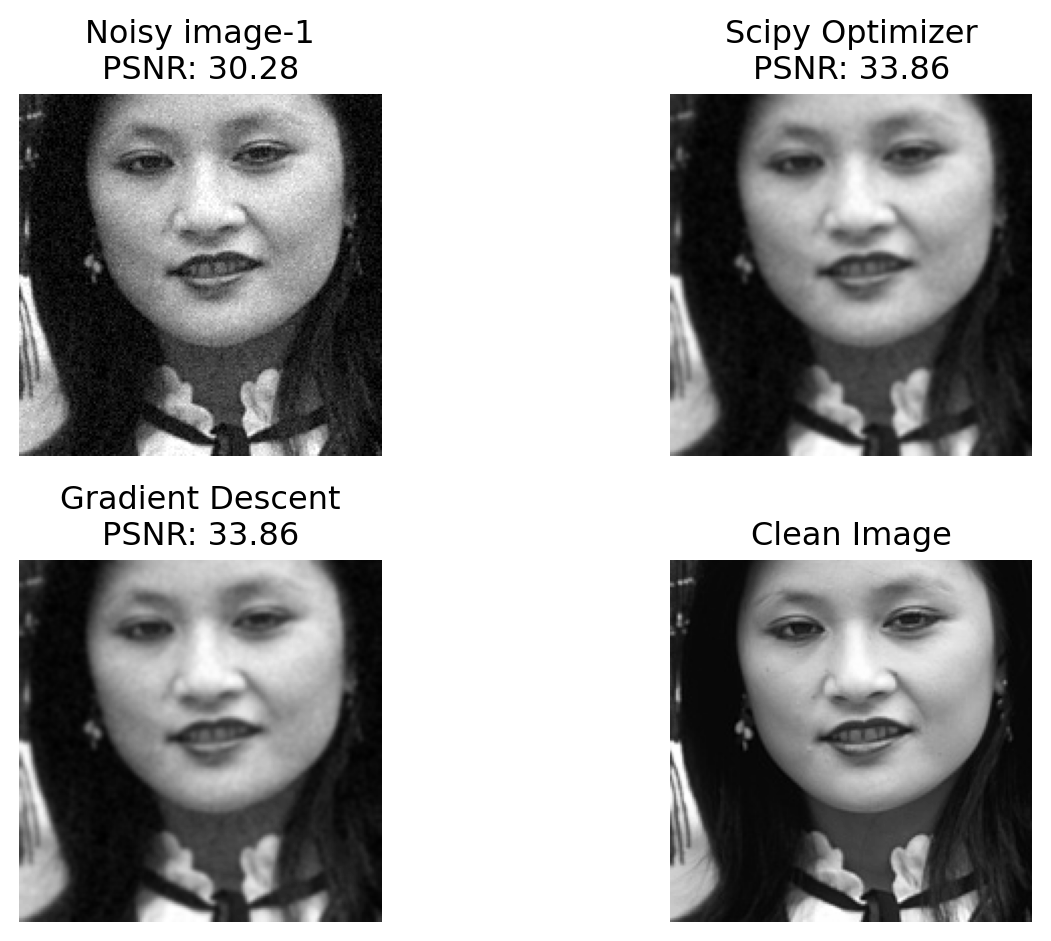
\includegraphics{index_files/figure-latex/notebooks-review-fig-denoising-plot-output-1.png}

}

\caption{\label{fig-denoising-plot}Example of denoising results.}

\end{figure}%

\textsubscript{Source:
\href{https://sijuswamy.github.io/Denoising-Manuscript/notebooks/review-preview.html\#cell-fig-denoising-plot}{Basics
of Noise}}

Skill of the proposed alogorithm on the same sample image used by the
author is shown in Figure~\ref{fig-denoising-plot}

\section{Conclusion}\label{conclusion}

The review examined several influential works that inspired the authors'
unsupervised denoising framework, including Noise2Noise (N2N), Noise as
Clean (NaC), and Noise2Noise Regression (Nr2N). These models
demonstrated how effective denoising can be achieved without relying on
clean ground-truth images, focusing solely on noisy data. By building on
these ideas, the authors introduced novel unsupervised cost functions
and inference schemes to match the performance of supervised denoising
models. Using Gaussian smoothing as a basic case study, the review
reproduced these methods and explored the optimization of the error
functions through scipy minimization and custom gradient descent.
Metrics such as MSE and PSNR provided a comparative analysis,
reinforcing that while the unsupervised method closely mirrors the
results of supervised models, further refinement is needed to fully
realize its potential in more complex scenarios.

\section{References}\label{references}

\phantomsection\label{refs}
\begin{CSLReferences}{1}{0}
\vspace{1em}

\bibitem[\citeproctext]{ref-4271520}
Dabov, K., Foi, A., Katkovnik, V., \& Egiazarian, K. (2007). Image
denoising by sparse 3-d transform-domain collaborative filtering.
\emph{IEEE Transactions on Image Processing}, \emph{16}(8), 2080--2095.
\url{https://doi.org/10.1109/TIP.2007.901238}

\bibitem[\citeproctext]{ref-9506794}
Dutta, S., Basarab, A., Georgeot, B., \& Kouamé, D. (2021a). Image
denoising inspired by quantum many-body physics. In \emph{2021 IEEE
international conference on image processing (ICIP)} (pp. 1619--1623).
\url{https://doi.org/10.1109/ICIP42928.2021.9506794}

\bibitem[\citeproctext]{ref-9382109}
Dutta, S., Basarab, A., Georgeot, B., \& Kouamé, D. (2021b). Quantum
mechanics-based signal and image representation: Application to
denoising. \emph{IEEE Open Journal of Signal Processing}, \emph{2},
190--206. \url{https://doi.org/10.1109/OJSP.2021.3067507}

\bibitem[\citeproctext]{ref-floquet:hal-04344047}
Floquet, A., Dutta, S., Soubies, E., Pham, D.-H., Kouamé, D., \& Kouame,
D. (2024). {Automatic Tuning of Denoising Algorithms Parameters without
Ground Truth}. \emph{{IEEE Signal Processing Letters}}, \emph{31},
381--385. \url{https://doi.org/10.1109/LSP.2024.3354554}

\bibitem[\citeproctext]{ref-knuth84}
Knuth, D. E. (1984). Literate programming. \emph{Comput. J.},
\emph{27}(2), 97--111. \url{https://doi.org/10.1093/comjnl/27.2.97}

\bibitem[\citeproctext]{ref-8954066}
Krull, A., Buchholz, T.-O., \& Jug, F. (2019). Noise2Void - learning
denoising from single noisy images. In \emph{2019 IEEE/CVF conference on
computer vision and pattern recognition (CVPR)} (pp. 2124--2132).
\url{https://doi.org/10.1109/CVPR.2019.00223}

\bibitem[\citeproctext]{ref-lehtinen2018noise2noise}
Lehtinen, J. (2018). Noise2noise: Learning image restoration without
clean data. \emph{arXiv Preprint arXiv:1803.04189}.

\bibitem[\citeproctext]{ref-9156650}
Moran, N., Schmidt, D., Zhong, Y., \& Coady, P. (2020). Noisier2Noise:
Learning to denoise from unpaired noisy data. In \emph{2020 IEEE/CVF
conference on computer vision and pattern recognition (CVPR)} (pp.
12061--12069). \url{https://doi.org/10.1109/CVPR42600.2020.01208}

\bibitem[\citeproctext]{ref-10222154}
Nguyen, P., Soubies, E., \& Chaux, C. (2023). Map-informed unrolled
algorithms for hyper-parameter estimation. In \emph{2023 IEEE
international conference on image processing (ICIP)} (pp. 2160--2164).
\url{https://doi.org/10.1109/ICIP49359.2023.10222154}

\bibitem[\citeproctext]{ref-9577798}
Pang, T., Zheng, H., Quan, Y., \& Ji, H. (2021).
Recorrupted-to-recorrupted: Unsupervised deep learning for image
denoising. In \emph{2021 IEEE/CVF conference on computer vision and
pattern recognition (CVPR)} (pp. 2043--2052).
\url{https://doi.org/10.1109/CVPR46437.2021.00208}

\bibitem[\citeproctext]{ref-4598837}
Ramani, S., Blu, T., \& Unser, M. (2008). Monte-carlo sure: A black-box
optimization of regularization parameters for general denoising
algorithms. \emph{IEEE Transactions on Image Processing}, \emph{17}(9),
1540--1554. \url{https://doi.org/10.1109/TIP.2008.2001404}

\bibitem[\citeproctext]{ref-7807310}
Selesnick, I. (2017). Total variation denoising via the moreau envelope.
\emph{IEEE Signal Processing Letters}, \emph{24}(2), 216--220.
\url{https://doi.org/10.1109/LSP.2017.2647948}

\bibitem[\citeproctext]{ref-9210208}
Xu, J., Huang, Y., Cheng, M.-M., Liu, L., Zhu, F., Xu, Z., \& Shao, L.
(2020). Noisy-as-clean: Learning self-supervised denoising from
corrupted image. \emph{IEEE Transactions on Image Processing},
\emph{29}, 9316--9329. \url{https://doi.org/10.1109/TIP.2020.3026622}

\bibitem[\citeproctext]{ref-5484579}
Zhu, X., \& Milanfar, P. (2010). Automatic parameter selection for
denoising algorithms using a no-reference measure of image content.
\emph{IEEE Transactions on Image Processing}, \emph{19}(12), 3116--3132.
\url{https://doi.org/10.1109/TIP.2010.2052820}

\end{CSLReferences}




\end{document}
